%%-------------------------Random process on sphere---------------------------------------%%

%%------------------------------------------------------------------%%
\section{Random process on a sphere}
%%------------------------------------------------------------------%%
	
Suppose $X \in \{X(P): P\in D\}$, defined in a common probability space $P \in S^2$ (unit sphere), where $P=(\lambda, \phi) \in S^2$ with longitude $\lambda \in [-\pi, \pi)$ and latitude $\phi \in [0, \pi]$. Suppose the process is isotropy and continuous in quadratic mean with respect to the location $P$ then the process can be represented by spherical harmonics, $P_{\nu}^m(\cdot)$ normalized associated Legendre polynomials, with the sum converges in mean square (\cite{Jones1963},\cite{LiNorth1997, Huang2012}).   
			
	\beq \nonumber
	X(P) = \sum_{\nu=0}^\infty \sum_{m=-\nu}^{\nu} Z_{\nu,m} e^{i m \lambda} P_{\nu}^m (\cos \phi),
	\eeq
			
	Since $\cos(\phi)\in[-1,1]$ we have $\int_{-1}^{1}[P_{\nu}^m(cos(\phi))]^2dcos(\phi) = 1$, and $Z_{\nu,m}$ are complex-valued coefficients satisfying.
			
	\beq \nonumber
	Z_{\nu,m} = \int_{S^2} X(P) e^{-im \lambda} P_{\nu}^m (\cos \phi) d P.
	\eeq
				
	Suppose the process $X(P)$ is isotropy with 0 mean (without loss of generality) which implies $E(Z_{\nu,m}) = 0$. Let $P = (\lambda_P, \phi_P)$ and $Q=(\lambda_Q, \phi_Q)$ be two arbitrary locations on the sphere, if the covariance function $R(P,Q)$ on $S^2$ solely depends on the spherical distance between $(P,Q)$,
	
	\begin{eqnarray*} \label{rpq_1}
		R(P, Q) &=& \mbox{E}(X(P) \overline{X(Q)}) \\
		&=& \sum_{\nu=0}^\infty \sum_{\mu=0}^\infty \sum_{m=-\nu}^{\nu} \sum_{n=-\mu}^{\mu} \mbox{E}(Z_{\nu,m} \overline{Z}_{\mu,n}) e^{im \lambda_P} P_{\nu}^m(\cos \phi_P) e^{-i n \lambda_Q} P_{\mu}^n (\cos \phi_Q).
	\end{eqnarray*}
				
	where $\bar{Z}$ denotes the complex conjugate of $Z$, $\theta_{PQ}$ is the spherical distance, $P_{\nu}(\cdot)$ is the Legendre polynomial. Note that the continuity of $X(P)$ on every point $P$ implies that $R(P, Q)$ is continuous at all pairs of $(P, Q)$ \cite[page 83]{Leadbetter1967}.
	
	
	%%------------------------------------------------------------------%%
	%\section{Covariance on sphere} 
	%%------------------------------------------------------------------%%
	
	Under the assumption of homogeneity (or isotropy) the random process $X(\cdot)$ on $S^2$ has a finite second moment and it is invariant under the rotations on the sphere with constant mean. Similarly, we can define an isotropic random process on a sphere as, 
	
	\begin{eqnarray*}
		E(X(s) &=& \mu \quad \mbox{for any } s\in S^2 \\
		Cov(X(P),X(Q)) &=& C(\theta_{PQ}) 
	\end{eqnarray*}
	
	where $\theta_{PQ}$ is the spherical angle between two locations $P,Q$. For a unit sphere, the distance between the two locations can be defined as great circle distance ($\gcd_{PQ}$) or chordal distance ($ch_{PQ}$) as follows,
	
	\begin{eqnarray*}
		\theta_{PQ}  &=& \arccos\left(\sin(L_1)\sin(L_2) + \cos(L_1)\cos(L_2)\cos(l_1-l_2)\right)\\
		% gcd_{PQ}    &=&  1\cdot\theta_{PQ}\\
		% ch_{PQ}     &=& 2\sin (\theta_{PQ}/2)
	\end{eqnarray*}
	
	In the case of $\R^d$, non-negative definite is a necessary and sufficient condition for a valid covariance function defined on $\R^d$ (\ref{cov_pd}). Similarly, a real continuous function $C(\cdot)$ defined on the sphere is a valid covariance function if and only if $C(\cdot)$ is non-negative definite,
	
	\beq
	\sum_{i,j=1}^{N} a_i a_j C(\theta_{PQ}) \ge 0,
	\eeq
	for any integer $N$, any constants $a_1, a_2, \ldots, a_N$, and any locations $P, Q, \ldots \in S^2$.\\
	
	Let $P_{k}^{\nu}(\cos\theta)$ be the ultraspherical polynomials defined by the following infinite summation,
	
	\beq
	\frac{1}{(1 - 2c\cos\theta + c^2)^{\nu}} = \sum_{k=0}^{\infty}c^{k} P_{k}^{\nu}(\cos\theta) \quad \nu>0
	\eeq
	
	
	\[
		\mbox{When $\nu = 0$, } P_{k}^{0}(\cos\theta) = \cos (k\theta)
	\]
	
	According to \cite{schoenberg1942}, a real continuous function $C(\theta)$ is a valid covariance function on $S^d$, where $d=1,2,\ldots$, if and only if it can be written in the following form
	
	\beq
	C(\theta) = \sum_{k = 0}^\infty c_kP_k^{(\nu)}(\cos\theta), \quad \nu=\frac{1}{2}(d-1)
	\eeq
	
	where $\forall c_k\ge 0$ and $\sum c_k < \infty$. \\
	
	Suppose $C(\cdot)$ is a covariance functions that is valid in $S^d$ then it is valid on $S^m$ where $d\le m$. In general we have the following property,
	
	\begin{eqnarray*}
		S^1 \subset S^2 \subset \cdots S^{d} \subset \cdots S^{\infty} \\
		C(S^1) \supset C(S^2) \supset \cdots C(S^d) \supset \cdots C(S^{\infty})
	\end{eqnarray*}
	
	and covariance functions that are valid on $S^m$ may not be valid on $S^d$ where $m>d$. \blue{should we add any examples?}\\
	
	In chapter 3 we discussed about the spectral representation of the covariance function on a circle 
	
	\[
		C(\theta) = \sum_{k = 0}^\infty c_k\cos (k\theta)
	\]
	
	It is easy to observe that $\cos\theta \in S^1$ and clearly $\cos\theta \in S^2$ and from the properties of covariance discussed in chapter 1, $P_k\cos\theta \in S^2$ where $P_k$ is a Legender polynomial. Therefore, when $d=2$ the covarince on a sphere ($S^2$) can be expressed as follows,
	
	\beq \label{covs2_sum}
	C(\theta) = \sum_{k = 0}^\infty c_kP_k(\cos\theta) \quad , c_k \ge 0
	\eeq
	
	% \blue{?if a covariance function is not valid on $S^r$ it is not valid on $S^d \quad d > r$ (example).}\\
	
	Since the Legendre polynomials are orthogonal we have
	
	\[
		\int_{-1}^{1} P_{n}(x)P_{m}(x)dx = \frac{2}{2n+1}\delta_{nm}
	\]
	
	and on a sphere the coefficients $c_k$ can be obtained by
	
	\beq \label{covs2_coef}
	c_{\nu} = \frac{2\nu+1}{2}\int_0^{\pi} C(\theta)P_{\nu}(\cos\theta)d\theta. \quad \nu = 0,1,2,\ldots
	\eeq
	
	One can directly use the above integral to evaluate the validity of a covariance function on the sphere by checking if $c_k$ is non-negative and $\sum c_k < \infty$ .\\ 
	
	All covariance models that are valid on $\R^d$ are not valid on the sphere ($S^2$), \cite{HuangZhangRobeson2011} evaluated the validity of commonly used covariance on a sphere that are valid on $\R^d$, they showed that some models are not valid on the sphere and some models are valid only for certain parameter values.  
	 
	
	\begin{table}[H]
		\label{valid_cov_models}
		\centering
		\begin{tabular}[htb]{lll} \hline \hline
			Model & Covariance function & Validity  $S^2$           \\   \hline Spherical  &
			$\left(1-\frac{3\theta}{2a} + \frac{1}{2}
			\frac{\theta^3}{a^3}\right){\bf 1}_{(\theta \le a)}$ & Yes   \\
			[2ex]
			Stable     & $\exp\left\{-\left(\frac{\theta}{a}\right)^\alpha\right\}$ & Yes for $\alpha \in (0,1]$  \\
			      &                     & No for $\alpha \in (1,2]$ \\ [2ex] \hspace{0.2in} Exponential &
			$\exp \{-\left(\frac{\theta}{a}\right) \}$ & Yes \\ [2ex]
			\hspace{0.2in} Gaussian & $\exp\left\{-\left(\frac{\theta}{a} \right)^2
			\right\}$  & No \\ [2ex]
			Power$^*$   & $c_0 - (\theta/a)^\alpha$ & Yes for  $\alpha \in (0,1] $  \\
			& & No for $\alpha \in (1,2]$ \\ [2ex]
			Radon transform of order 2         & $e^{-\theta/a}(1+\theta/a)$ &
			No        \\ [2ex] Radon transform of order 4         &
			$e^{-\theta/a} (1+\theta/a+\theta^2/3a^2)$  & No  \\ [2ex] Cauchy &
			$(1+\theta^2/a^2)^{-1}$ &  No      \\ [2ex] Hole - effect & $\sin
			a\theta / \theta$ & No    \\ \hline \hline
		\end{tabular}
		\caption{Validity of covariance functions on the sphere, $a >
			0,\theta \in [0,\pi]$. $^*$When $\alpha \in (0,1]$, power model is
				valid on the sphere  for some $c_0 \ge \int_0^\pi
				(\theta/a)^{\alpha} \sin \theta d \theta$.} \label{tab:t1}
							
		\end{table}
			
		Furthermore, \cite{Gneiting2013} argued that Mat$\acute{e}$rn covariance function is valid on the sphere when the smoothness parameter $\nu\in(0,1/2)$ and it is not valid if $\nu>1/2$. \cite{Yadrenko1983} showed that if $K(\cdot)$ is valid isotropic covariance function on $\R^3$ then
			
		\[
			C(\theta) = K(2\sin(\theta/2))
		\]
			
		is a valid isotropic covariance function on the unit sphere (where $\theta$ is $gcd$).\\
			
		%%------------------------------------------------------------------%%
		%\section{Variogram on a sphere}
		%%------------------------------------------------------------------%%
			
			
		Similar to the case of circle, if a random process $X(\cdot)$ on a sphere is intrinsically stationary on $S^2$, then one has $E(X(P))=\mu$ an unknown constant for all $P\in S^2$ and the variogram function between any two locations $P, Q \in S^2$ depends only on the spherical angle $\theta_{PQ}$ 
			
		\[
			Var(X(P)-X(Q)) = 2\gamma(\theta_{PQ}) \quad , \forall P, Q \in S^2
		\]
			
		The variogram is conditionally negative definite
			
		\[
			\sum_{i,j=1}^{N} a_i a_j 2\gamma(\theta_{PQ}) \le 0,
		\]
			
		for any integer $N$, any constants $a_1, a_2, \ldots, a_N$ with $\sum a_i = 0$, and any locations $P, Q, \ldots \in S^2$. Immediately from \ref{covs2_sum} for a continuous $2\gamma(\cdot)$ with $\gamma(0)=0$ the variogram is negative definite if and only if 
			
		\beq 
		\gamma(\theta) = \sum_{k = 0}^\infty c_k(1-P_k(\cos\theta))
		\eeq
		where $P_{k}(\cdot)$ are Legendre polynomials with $\forall c_k\ge 0$ and $\sum c_k < \infty$. \\
			
		In the introduction we pointed out in $\R^d$ one can always construct the variogram if the covariance function is given but not the converse. However, in $S^2$ \cite{Yaglom1961} argued that for a valid $\gamma(\theta) \quad \theta \in [0,\pi]$ one can always construct covariance function $C(\theta)=c_0-\gamma(\theta)$ for some $c_0 \ge \int_0^{\pi} \gamma(\theta)\sin(\theta)d\theta$. 
			
		
		%%------------------------------------------------------------------%%
		\section{Axially symmetry}
		%%------------------------------------------------------------------%%
					
		All covariance models that are valid on $R^3$ are not valid on $S^2$ and it is necessary to use $S^2$ instead of $R^3$ when studying about random processes on Earth and isotropy is often assumed (\cite{Yadrenko1983, Yaglom1987}). However, many studies have pointed out this assumption is not reasonable (\cite{Stein2007, JunStein2008, BolinLindgren2011}) for random processes on the sphere primarily on Earth. \cite{Stein2007} argued that Total Ozone Mapping Spectrometer (TOMS) data varies strongly with latitudes and homogeneous models are not suitable. Moreover, aerosol depth (AOD) from Multi-angle Imaging Spectrometer (MISR), Sea Surface Temperature (SST) from RRMM Microwave Imager (TMI) are some other example for anisotropy global data on a sphere (on Earth). In order to study non homogeneous processes on the sphere \cite{Jones1963} introduces the concept of axially symmetry, where the covarince between two spatial points depend on the longitudes only through their difference  between two points.
					
		A random process $X(P): P\in S^2$ on the sphere and let $R(P,Q)$ be a valid covarince function on the sphere where $P=(L_P, l_P), Q(L_Q,l_Q)$ then $X(P)$ is axially symmetric if and only if
				
		\[
			R(L_P, L_Q, l_P, l_Q) = R(L_P, L_Q, l_P-l_Q).
		\]
				
		Currently, to our knowledge there are no methods to test axially symmetry in real data. However, this assumption is more plausible and reasonable when modeling spatial data. For example, temperature, moisture, etc. most likely symmetric on longitudes rather than latitudes. \cite{Stein2007} propose a method to model axially symmetric process on a sphere (the fitted model is not the best, but this was a good start). When modeling spatial data stationary models are less useful; but using the concept of axially symmetry \cite{JunStein2008} proposed a flexible class of parametric covariance models to capture the non-stationarity of global data. \cite{HitczenkoStein2012} discussed about the properties of an existing class of models for axially symmetric Gaussian processes on the sphere. They applied first-order differential operators to an isotropic process. \cite{Huang2012} developed a new representation of axially symmetric process on the sphere and further introduced some parametric covariance models that are valid on $S^2$.  \\
				
		if the process is axially symmetric $E(Z_{\nu,m} \overline{Z}_{\mu,n})$ can be expressed as,
				
		\[
			\mbox{E} (Z_{\nu,m} \overline{Z}_{\mu,n}) = \delta_{n,m} f_{\nu,\mu,m}.
		\]
					
		Hence, for an axially symmetric process the covariance function (\ref{rpq_1}) will be the following form (\cite{Huang2012}) 
					
		\begin{eqnarray} \label{axially-symmetry-cov}
			R(P,Q)  & = & R(\phi_P, \phi_Q, \lambda_P-\lambda_Q) \nonumber \\
			& = & \sum_{m=-\infty}^{\infty} \sum_{\nu=|m|}^\infty \sum_{\mu=|m|}^\infty f_{\nu,\mu,m} e^{im (\lambda_P-\lambda_Q)} P_{\nu}^m(\cos \phi_P) P_{\mu}^m (\cos \phi_Q) .
		\end{eqnarray}
					
		In order to have a valid covariance function, $f_{\nu,\mu, m} = \overline{f}_{\mu, \nu, m}$ and for each fixed integer $m$, the matrix $F_m(N) = \{ f_{\nu,\mu,m} \}_{\nu,\mu=|m|,|m|+1, \ldots, N }$ must be positive definite for all $N \ge |m|$. 
				
		\beq \label{R(PQ)-01}
		R(P,Q) = R(\phi_P,\phi_Q,\Delta\lambda) = \sum_{m = -\infty}^{\infty}e^{im\Delta\lambda}C_m(\phi_P,\phi_Q) \quad m=0, \pm 1, \pm 2,...
		\eeq
				
		where $\Delta\lambda \in [-\pi, \pi]$ and $\phi_P, \phi_Q \in [0,\pi]$
		%-------------------------------------%
		\subsection{Properties of \Cm}
		%-------------------------------------%
					
		The covariance function $R(P,Q)$ based on the concept of axially symmetry is clearly defined by both latitudes and longitudes (difference). The following conditions for \Cm are very important to have a valid covariance function defined by \ref{R(PQ)-01}.  
					
		\begin{itemize}
			\item Hermitian and positive definite.
			\item $\sum_{m = -\infty}^{\infty}|C_m(\phi_P,\phi_Q)|<\infty$ for $m=0,\pm 1, \pm  2$, ...
			\item Is a continuous function. 
		\end{itemize}
				
		% %-------------------------------------% 
		% \begin{thm}[Mercer's theorem (simplified version) ] \hfill \\
		% 	%-------------------------------------% 
		% 	
		% 	A kernal $K:[a,b]\times [a,b] \to \R$ be a symmetric continuous function that is non-negative definite,
		% 	
		% 	\[
		% 		\sum_{i=1}^{n}\sum_{j=1}^{n} a_i a_j K(s, t) \ge 0 \quad \mbox{and} \quad K(s,t) = K(t,s)
		% 	\]
		% 	
		% 	for all $(s,t)\in [a,b]$ and $a_i>0$. Let $T_K:L_2 \to L_2$ be an intergral operator defined by
		% 	
		% 	\[
		% 		[T_Kf](\cdot) = \int_{a}^{b} K(\cdot,s)f(s)ds
		% 	\]
		% 	
		% 	is positive, for all $f\in L_2$
		% 	
		% 	\[
		% 		\int_{a}^{b} K(s, t)f(s)f(t)dsdt \ge 0.
		% 	\]
		% 	
		% 	The corresponding orthonormal eigen functions $\psi_i\in L_2$ and non negative eigen values $\lambda_i \ge 0$ of the operator $T_k$ is defined as
		% 	
		% 	\[
		% 		T_K(\psi_i(\cdot)) = \int K(\cdot, s)\psi(s)ds = \lambda_i\psi_i(\cdot), \quad \int \psi_i(\cdot)\psi_j(\cdot) = \delta_{ij}
		% 	\]
		% 	
		% 	
		% 	then the kernal $K(\cdot)$ is a uniformly convergent series in terms of eigen functions and associated eigen values of $T_k$ as follows,
		% 	
		% 	\[
		% 		K(s,t) = \sum_{j=1}^{\infty} \lambda_i \psi_i(s)\psi_i(t) 
		% 	\]
		% 	
		% \end{thm}
				
		One can use inverse Fourier transformation to derive $C_m$ based on an axially symmetric covariance function $R(P,Q)$ defined on a sphere, as we have
				
		\[ 
			C_m(\phi_P, \phi_Q) = \frac{1}{2\pi}\int_{-\pi}^{\pi} R(\phi_P, \phi_Q)e^{-im\Delta\lambda} d\Delta\lambda \]
				
			% Since \Cm is continuous and both Hermitian and positive definite, Mercer's theorem (\ref{mercer}) can be directly applied to \Cm such that there exists an orthonormal basis $\{\psi_{m,\nu}, \nu = 0,1,\ldots \}$ in $L^2$ (\cite{Huang2012}) and \Cm can be given by, 
				
			% 	\[ 
			% 	C_m(\phi_P,\phi_Q) = \sum_{\nu=0}^{\infty} \eta_{m,\nu}\psi_{m,\nu}(\phi_P)\overline{\psi_{m,\nu}(\phi_Q)},  \]
			% 	
			% 	% Where $\eta_{m,\nu}\ge 0$ and $\psi_{m,\nu}(\cdot)$ are the corresponding eigen values and eigen functions for \Cm.\\
			% 
			% Now the covariance function on a sphere is given by,
			% 		\beq \label{RPQ_orthonormal}
			% 			R(P,Q) = \sum_{m=-\infty}^{\infty}\sum_{\nu=0}^{\infty} \eta_{m,\nu}e^{im\Delta\lambda}\psi_{m,\nu}(\phi_P)\overline{\psi_{m,\nu}(\phi_Q)},
			% 		\eeq
			% 		
			% 		Where $\Delta\lambda \in [0, \pi]$, $\eta_{m,\nu}\ge 0$ and $\psi_{m,\nu}(\cdot)$ are the eigen values eigen functions of $C_m(\phi_P, \phi_Q)$ respectively.
					
			
					
			Let's consider a real-valued process with a complex valued \Cm as given below,
			
			\begin{eqnarray*}
				C_m(\phi_P,\phi_Q) &=& c_m f(\phi_P,\phi_Q)e^{i\omega_m(\phi_P-\phi_Q)}, \quad c_m \ge 0,\omega_m\in R \\
				&=& c_mC_m^{R}(\phi_P,\phi_Q) + i c_mC_m^{I}(\phi_P,\phi_Q).
			\end{eqnarray*}
			
			\cite{Huang2012} states that if a process is real-valued then the corresponding covariance function $R(P,Q)$ is also real-valued and \Cm $= \overline{C_{-m}(\phi_P,\phi_Q)}$, The covarince function $R(P,Q)$ on the sphere given by \ref{R(PQ)-01} can be simplified to the following form,
					
			
			\begin{eqnarray*}
				R(P,Q) &=& C_0(\phi_P,\phi_Q) + \sum_{m=1}^{\infty} e^{-im\Delta\lambda}C_{-m}(\phi_P,\phi_Q) +  \sum_{m=1}^{\infty} e^{im\Delta\lambda}C_m(\phi_P,\phi_Q) \\ 
				% &=& C_0(\phi_P,\phi_Q) + \sum_{m=1}^{\infty} c_m e^{-im\Delta\lambda}( C_m^{R}(\phi_P,\phi_Q) - i C_m^{I}(\phi_P,\phi_Q)) \\
				% & &  + \sum_{m=1}^{\infty}c_m e^{im\Delta\lambda}( C_m^{R}(\phi_P,\phi_Q) + iC_m^{I}(\phi_P,\phi_Q)) \\ 
				&=& c_oC_{0}^{R}(\phi_P,\phi_Q)+2 \sum_{m=1}^{\infty}c_m[\cos(m\Delta\lambda)C_{m}^{R}(\phi_P,\phi_Q)-\sin(m\Delta\lambda)C_{m}^{I}(\phi_P,\phi_Q)].
			\end{eqnarray*}
			
			
			There are several covariance models, $R(P,Q)$, valid on a sphere suggested by \cite{Huang2012}  carefully choosing values for $c_m$.
					
					
			\begin{table}[H]
				\centering
				\begin{tabular}{l|l|l}
					\hline
					Model   & $c_m$                                         & parameters                               \\ 
					\hline \hline
					model 1 & : $c_m = Cp^m  \mbox{ and } c_0 = C$          & $m=0, \pm 1, \pm 2,... \quad p\in (0,1)$ \\
					model 2 & : $c_m = \frac{Cp^m}{m} \mbox{ and } c_0 = 0$ & $m=\pm 1, \pm 2,... \quad p\in (0,1)$    \\
					model 3 & : $c_m = \frac{C}{m^4} \mbox{ and } c_0 = 0$  & $m=\pm 1, \pm 2,...$                     \\
					\hline
				\end{tabular}
				\label{Cm_table}
				\caption{some proposed $c_m$ models}
			\end{table}
						
			%%------------------------------------------------------------------%%
			%\section{Longitudinally reversibile process}
			%%------------------------------------------------------------------%%
						
			Suppose $K(\cdot)$ is a valid covariance function defined on a sphere where,
			
			\beq
			K(L_1, L_2, l_1-l_2 = K(L_1, L_2, l_2-l_1)
			\eeq
			
			is special a case for axially symmetric process and the underline process is said to be longitudinally reversible, the idea was first introduced by \cite{Stein2007}.  
			
			For example the covariance model proposed by \cite{Huang2012} clearly yields a longitudinally reversible process as $R(\phi_P, \phi_Q, \Delta\lambda) = R(\phi_P, \phi_Q, -\Delta\lambda)$ and the reversibility holds when $C_{-m}(\phi_P,\phi_Q)=C_m(\phi_P,\phi_Q)$. Now the covariance function reduces to the following,  
			
			\[
				R(P,Q) = \sum_{m=0}^{\infty} C_m(\phi_P,\phi_Q)\cos(m\Delta\lambda)
			\]
			
			If a random process on the sphere is real valued and longitudinally reversible so is the covariance function, $R(P,Q),$ is real valued then \Cm is real since $C_{-m}(\phi_P,\phi_Q)=C_m(\phi_P,\phi_Q)$  and \Cm $= \overline{C_{-m}(\phi_P,\phi_Q)}$.
			
				
			%%------------------------------------------------------------------%%
			\section{Generalization of parametric models}
			%%------------------------------------------------------------------%%
					
			\blue{How to discuss/link about other parametric models suggested by \cite{JeongJun2015}, \cite{JunStein2008}, etc... and why are we using \cite{Huang2012} and what are the advantages?} \\
					
			The covariance function on sphere, $R(P,Q)$,  given in equation \ref{R(PQ)-01}, is clearly a function of both longitude and latitude. 
			% \cite{Huang2012} pointed out that the simplest model is the separable model can be defined as follows,
				
			\[
				R(P,Q) = f(\Delta\lambda, \phi_P,\phi_Q)
			\]
					
			In order to make things easier one could assume that $C_m(\phi_P, \phi_Q) = \tilde{C}_m(\phi_P - \phi_Q)$ only depends on the difference of $\phi_P$ and $\phi_Q$, \cite{HuangZhangRobeson2011} proposed a simple separable covariance function when both covariance components are exponential
			\[
				R(P, Q) = c_0e^{-a|\Delta \lambda|}e^{-b|\phi_P - \phi_Q|},
			\]
					
			Where $a$ and $b$ are defined as decay parameters in longitude and latitude respectively. The separable models are too simple and they are not capable to capture the covariance structure of the entire sphere. Therefore, \cite{Huang2012} proposed some non-separable covariance models by carefully choosing functions for $C_m(\phi_P, \phi_Q)$  that are valid on the sphere,
					
			\begin{eqnarray}
				R(P,Q) &=& Ce^{-a|\phi_P-\phi_Q|} \frac{1-p^2}{1-2p \cos\Theta+p^2} \label{model1} \\
				R(P,Q) &=& Ce^{-a|\phi_P-\phi_Q|} \log\frac{1}{(1-2p\cos\Theta* + p^2)} \label{model2} \\
				R(P,Q) &=& 2Ce^{-a|\phi_P-\phi_Q|}\left(\frac{\pi^4}{90}-\frac{\pi^2\Theta^2}{12}+\frac{\pi\Theta^3}{12}-\frac{\Theta^4}{48}\right), \label{model3}
			\end{eqnarray}
			
			where $\Theta = \Delta\lambda + u(\phi_P - \phi_Q) - 2k\pi$, and $k$ is chosen such that $\Theta \in [0,2\pi]$.\\
			
			There is one big disadvantage of the covariance models proposed by \cite{Huang2012}, the biggest disadvantage for all of them are that it is assumed not only stationarity on longitudes, but stationarity on latitudes as well. \\
			
			We have noticed that when $\phi_P = \phi_Q$, the model \ref{model1} reduces to
			\beq
			\nonumber
			R(P, P) = C\frac{1-p^2}{1 - 2p\cos(\Delta\lambda)+p^2}
			\eeq
			and if we set $\Delta \lambda = 0$, the variance of latitude $\phi_P$ over all latitudes can be given by,
			\beq
			\nonumber
			Var(P) = C\frac{1+p}{1 - p}
			\eeq
					      		      
			is not a function of the latitude (a function of the parameter $p$) and it implies that variance is constant over all latitudes. This is not supposed to be the case, since both MSU data and TOMS data in figures \ref{MSU_data_var_lat} and \ref{TOMS_data_var_lat} shows that variance is highly depending on the latitude. In order to overcome this issue we propose a solution to the above covariance models to capture the non stationarity over the latitudes.		      
			
			\begin{prop} \label{prop_nonstationary_cov}
				%\prop\hfill\\
				A more general non stationary covariance function is given as following. If $C(\cdot) = C(x-y)$ is the stationary covariance function and $f(\omega) \ge 0$ is the corresponding spectral density, then
				\[
					\tilde{C}(x, y) = C_2 - C(x) - C(y) + C(x-y), 
				\]
				with 
				\[
					C_2 \ge \int_{-\infty}^\infty dF(\omega) = \int_{-\infty}^\infty f(\omega)d\omega > 0
				\]
				is the non stationary covariance function. Note that the covariance function $C(\cdot)$ implies that, by Bochner's theorem, there exists a bounded measure $F$ such that
				\[
					C(x) = \int_{-\infty}^\infty e^{-ix\omega}dF(\omega).
				\]
				When $F(\cdot)$ is absolutely continuous, there exists a spectral density $f(\cdot) \ge 0$ such that
				\[
					C(x) = \int_{-\infty}^\infty e^{-ix\omega}f(\omega)d\omega.
				\]
				Now we choose a sequence of complex numbers $a_i, i = 1, 2, \cdots, n$, and any sequence of real numbers $t_i, i = 1, 2, \cdots, n$, taking $C_2 = \int_{-\infty}^\infty f(\omega)d\omega$,
				\begin{eqnarray*}
					\sum_{i=1}^n \sum_{j=1}^n a_i \overline{a}_j \tilde{C}(t_i, t_j) &=& \sum_i \sum_j a_i \overline{a}_j (C_2 - C(t_i) - C(-t_j) + C(t_i-t_j)) \\
					&=& \sum_{i=1}^n \sum_{j=1}^n a_i \overline{a}_j \int_{-\infty}^\infty(1-  e^{-it_i\omega} - e^{it_j\omega} + e^{-i(t_i-t_j)\omega})f(\omega)d\omega \\
					&=&\int_{-\infty}^\infty f(\omega)d\omega \left|\sum_{i=1}^n a_i(e^{-it_i\omega} - 1)\right|^2 \ge 0.
				\end{eqnarray*}
			\end{prop}
					
			
			
			In the case of circle clearly $C_1e^{|\theta|}$ is a stationary covariance function and we can apply \ref{prop_nonstationary_cov} to get a non stationary covariance function. Lets consider the following stationary covariance functions over the latitudes,
					      		
			\begin{eqnarray*}
				C(\phi) = Ce^{-a|\phi_P|} \\
				C(\phi) = C\frac{1}{\sqrt{a^2+\phi^2}}
			\end{eqnarray*}
			
			Now, we apply proposition \ref{prop_nonstationary_cov} to get non-stationary covariance functions, which depends on the latitudes, even when $\phi_P = \phi_Q$. Consider the below two functions for \Cm.
					      		      
			\begin{eqnarray}
				\label{Cm_model1}
				\tilde{C}(\phi_P, \phi_Q) &=& C_1(C_2 - e^{-a|\phi_P|} - e^{-a|\phi_Q|} + e^{-a|\phi_P - \phi_Q|}) \\
				\label{Cm_model2}
				\tilde{C}(\phi_P, \phi_Q) &=& C_1\left(C_2 - \frac{1}{\sqrt{a^2+\phi_P^2}} - \frac{1}{\sqrt{a^2+\phi_Q^2}} + \frac{1}{\sqrt{a^2+(\phi_P-\phi_Q)^2}}\right)
			\end{eqnarray}
					      		      
			Here $C_1, a > 0,$ and $C_2 \ge 1$ to ensure the positive definiteness of the above function. When $\phi_P = \phi_Q$, both functions are actually a function of $\phi_P$.
					      		      
			\begin{eqnarray*}
				\tilde{C}(\phi_P, \phi_P) &=& C_1(C_2 - 2e^{-a|\phi_P|} + 1), \\
				\tilde{C}(\phi_P, \phi_P) &=& C_1\left(C_2 - \frac{2}{\sqrt{a^2+\phi_P^2}} + \frac{1}{a}\right).
			\end{eqnarray*}
			
			
					
			So we propose six five-parameter models which are combinations of both $\tilde{C}(\phi_P, \phi_Q)$, defined by a exponential family \ref{Cm_model1} and a power family \ref{Cm_model2}, and models (\ref{model1}, \ref{model2}, \ref{model3}) proposed by \cite{Huang2012} for the covariance on a sphere defined as follows,
					
			\[
				R(P,Q) = \tilde{C}(\phi_P, \phi_Q) C(\Theta),
			\]
			where $\Theta=\Delta\lambda+u(\phi_P-\phi_Q) \in [0,2\pi ] $, $C_1 > 0, C_2 > 0, a>0, u\in \R, p\in(0,1)$. 
					
			\begin{figure}[H]
				\centering
				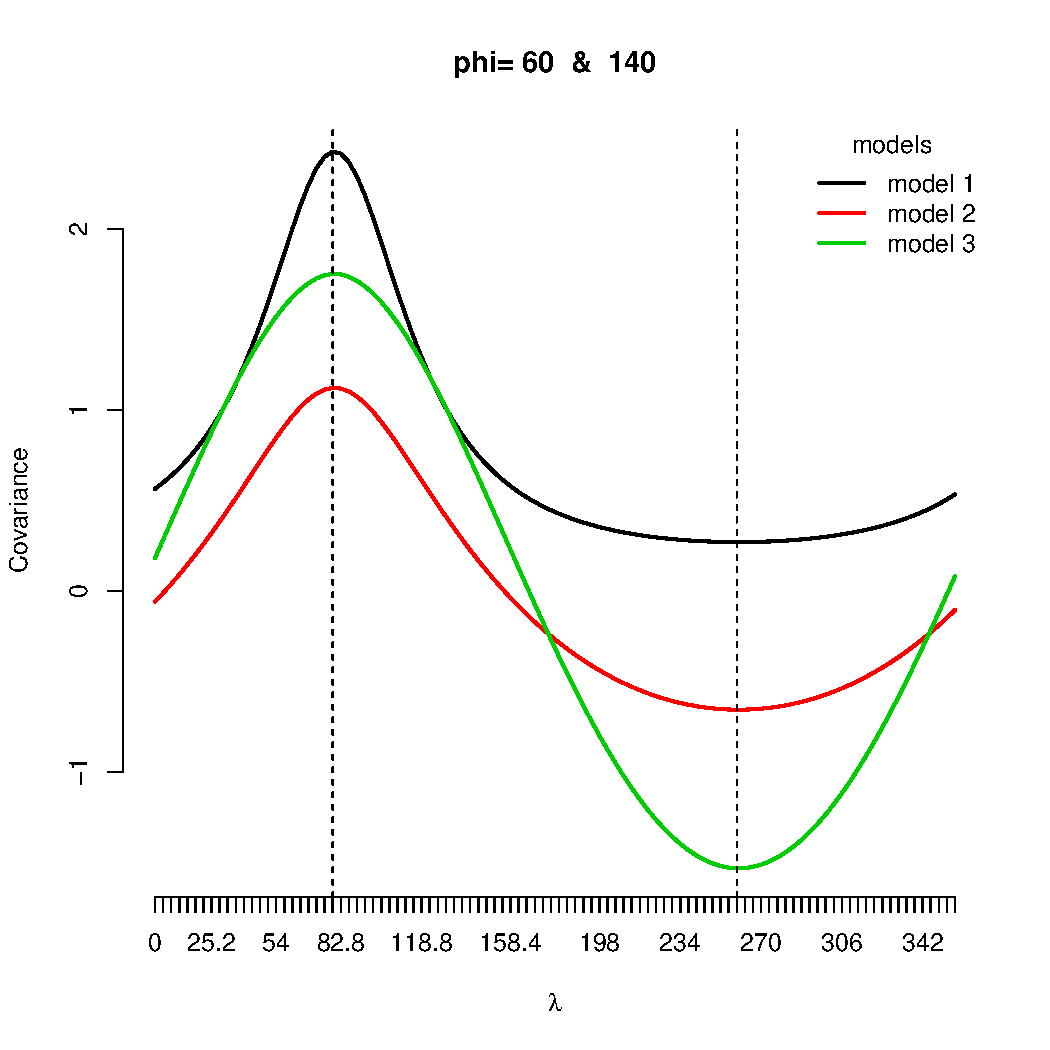
\includegraphics[width=0.9\textwidth]{graphs/all_covariance_models}
				\caption[The covariance between $30^0S$ and $50^0N$ (latitude $60^0$ and $140^0$) of three covariance models] {The covariance between $30^0S$ and $50^0N$ (latitude $60^0$ and $140^0$) of three covariance models with exponential family $ i.e. \tilde{C}(\phi_P, \phi_Q)$ given by \ref{Cm_model1} over 100 longitudes  for simplicity we set all parameters to be one.}
			\end{figure}
				
			{\bf Remark 1} The parameters $C_1, C_2, a, p$ are scaling parameters of the covariance functions and $u$ is a location parameter. All covariance models have a similar pattern and share one property, when there is no location shift ($u = 1$) the maximum of $R(P,Q)$ occurs at $\lambda_{max} = |\phi_P -\phi_Q|$ and the minimum of $R(P,Q)$ occurs at $\lambda_{min} = \pi + \lambda_{max}$. 
					
			\begin{figure}[H]
				\centering
				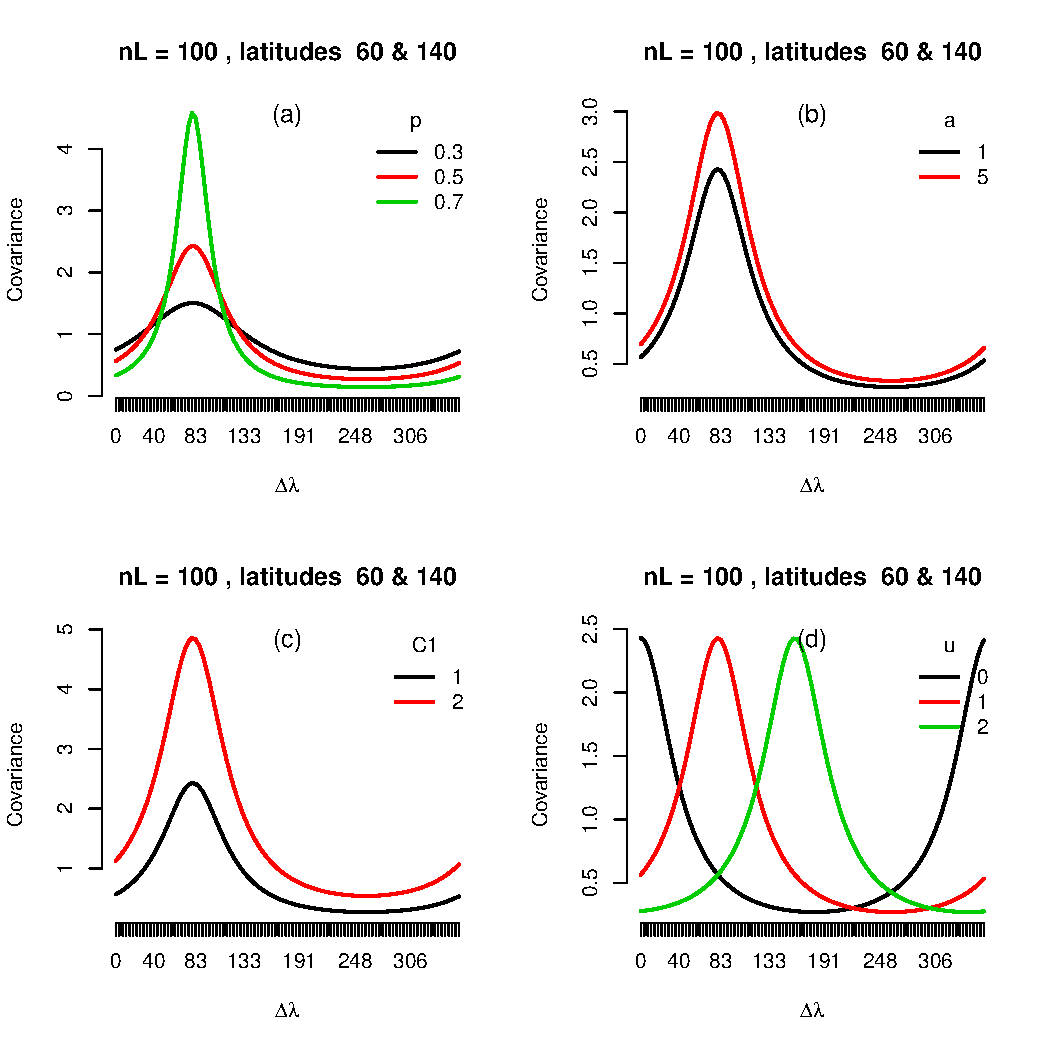
\includegraphics[width=0.9\textwidth]{graphs/parameters_model1_2}
				\caption[Covariance distribution for different parameters using model1:] {Covariance distribution for different parameter using model1:  (a)-parameter $p$, (b)-parameter $a$, (c)-parameter $C1$ (similar pattern for parameter $C2$), (d)-parameter u}
				\label{fig_parameter_comp}
			\end{figure}
			
			{\bf Remark 2} The scaling parameter $p$ is more sensitive at supremum and infimum of the covariance models and parameters $C_1, C_2, a$ are regular scaling parameters. The parameter $u$ is a location parameter which shits the covariance from left to right ($\Delta\lambda$) when $u>0$, but $u=0$ will provide a longitudinally reversible covariance model which is similar to Mat$\acute{e}$rn covariance model when the smoothing parameter ($\nu$) is 1/2.  \\     
			
			
			%%------------------------------------------------------------------%%
			\section{Covariance and variogram estimators on a sphere}
			%%------------------------------------------------------------------%%
			%In contrast the cross variogram is an even function when the process is intrinsically stationary. 
				
			\subsubsection{Cross Covariance}
					
			The cross covariance captures the covarince between two locations and any finite pairs of locations separated by a fixed distance (longitudinal difference $\Delta\lambda$). In other words cross covariance can be used to to capture the covariance between points at two latitudes separated by $\Delta \lambda \in (0,2\pi)$. When a axially symmetric random process on a sphere is second-order stationary, cross covariance is a function of longitudinal difference ($\Delta\lambda$). According to \cite{Wackernagel2013} the cross covariance function is not an even function and it is easy to observe that the proposed $R(P,Q)$ functions are valid on a sphere and they are cross covarince functions ($R(P,Q, \Delta\lambda) \ne R(P,Q,-\Delta\lambda)$). 
			The cross covariance estimate for axially symmetric processes on the sphere. For any two latitudes $\phi_P$ and $\phi_Q$ with $\{\lambda_i, i = 1, 2, \ldots, n\}$ representing the gridded longitudes on each circle, then $\hat{R}(\phi_P, \phi_Q, \Delta \lambda)$ is given by
					
			% 	\beq \label{emprical_var}
			% 	\hat{R}(\phi_P, \phi_Q, \theta) = \frac{1}{n_L}\sum_{k=1}^{n_L}(X(\phi_P, \theta+\lambda_k)\cdot X(\phi_Q, \lambda_k)),
			% 	\eeq
			% 	where $\theta = m\Delta\lambda$.
			% 	
			% In general, the spatial processes are stationary at a given latitude but not within latitudes. 
				
			%If the processes are not zero mean once could simply substract the product of means from the above MOM estimator.
			% 
			% The above estimate is clearly unbiased as we have, for fixed two locations $P, Q \in S^2$,
			% \[
			% 	E[\hat{R}(\phi_P, \phi_Q, \theta)] = R(P,Q).
			% \]
			% 
			% Later we will prove this estimator is consistent, {\em i.e.,} for any $\varepsilon > 0$,
			% \[
			% 	\lim_{n \to \infty} P(|\hat{R}(\phi_P, \phi_Q, \theta) - R(P,Q)| > \varepsilon) = 0.
			% \]
					
			\beq
			\hat{R}(\phi_P, \phi_Q, \Delta \lambda)= \frac{1}{n}\sum_{i = 1}^n (X(\phi_P, \lambda_i + \Delta \lambda) - \bar{X}_P)(X(\phi_Q, \lambda_i) - \bar{X}_Q), 
			\eeq
				
			where $\Delta \lambda = 0, 2\pi/n, 4\pi/n, \cdots, 2(N-1)\pi/n$ and $\bar{X}_P = \frac{1}{n}\sum_{i=1}^n X(\phi_P, \lambda_i)$ and similar for $\bar{X}_Q$. Now we calculate the unbiasedness of the cross covarince estimator. 
				
			\begin{eqnarray*}
				E(\hat{R}(\phi_P, \phi_Q, \Delta \lambda)) &=& \frac{1}{n}\sum_{i = 1}^n E((X(\phi_P, \lambda_i + \Delta \lambda) - \bar{X}_P)(X(\phi_Q, \lambda_i) - \bar{X}_Q)) \\
				&=& \frac{1}{n}\sum_{i=1}^n cov(X(\phi_P, \lambda_i+\Delta \lambda), X(\phi_Q, \lambda_i)) \\
				& & - \frac{1}{n}\sum_{i = 1}^n E((X(\phi_P, \lambda_i + \Delta \lambda) - \mu_P)(\bar{X}_Q - \mu_Q)) \\
				& & -\frac{1}{n}\sum_{i = 1}^n E((X(\phi_Q, \lambda_i) - \mu_Q)(\bar{X}_P - \mu_P)) \\
				& & + \frac{1}{n}\sum_{i = 1}^n E((\bar{X}_P - \mu_P)(\bar{X}_Q - \mu_Q)) \\
				&=& R(\phi_P, \phi_Q, \Delta \lambda) -E((\bar{X}_Q - \mu_Q)(\bar{X}_P - \mu_P)) - E((\bar{X}_P - \mu_P)(\bar{X}_Q - \mu_Q)) \\
				& &  + E((\bar{X}_P - \mu_P)(\bar{X}_Q - \mu_Q)) \\
				&=& R(\phi_P, \phi_Q, \Delta \lambda) - cov(\bar{X}_P, \bar{X}_Q).
			\end{eqnarray*}
				
			Note that, 
				
			\begin{eqnarray*}
				cov(\bar{X}_P, \bar{X}_Q) &=&  \frac{1}{n^2}\sum_{i = 1}^n \sum_{j=1}^n cov(X(\phi_P, \lambda_i), X(\phi_Q, \lambda_j)) \\
				&=& \frac{1}{n^2}\sum_{i = 1}^n \sum_{j=1}^n R(\phi_P, \phi_Q, (i-j)*2\pi/n) \\
				&=& \frac{1}{n^2}\sum_{i = 1}^n \sum_{j=1}^n \left( C_0(\phi_P, \phi_Q) \right.\\
				& &  2\sum_{m=1}^\infty \left( C_{m, R}(\phi_P, \phi_Q) \cos(m*(i-j)*2\pi/n) \right. \\
				& & \left.- C_{m, I}(\phi_P, \phi_Q) \sin(m*(i-j)*2\pi/n) \right) \\
				&=& C_0(\phi_P, \phi_Q) + 2\sum_{m=1}^\infty C_{m, R}(\phi_P, \phi_Q) \left(\frac{1}{n^2}\sum_{i = 1}^n \sum_{j=1}^n \cos(m(i-j)*2\pi/n)\right) \\
				& & - 2\sum_{m=1}^\infty C_{m, I}(\phi_P, \phi_Q) \left(\frac{1}{n^2}\sum_{i = 1}^n \sum_{j=1}^n \sin(m(i-j)*2\pi/n)\right) \\
				&=& C_0(\phi_P, \phi_Q),
			\end{eqnarray*}
				
			since
			\begin{eqnarray*}
				& & \sum_{i = 1}^n \sum_{j=1}^n \cos(m*(i-j)*2\pi/n) \\
				&=& \sum_{i=1}^n \sum_{j=1}^n \left(\cos(m*i *2\pi/n)\cos(m*j*2\pi/n) - \sin(m*i *2\pi/n)\sin(m*j*2\pi/n) \right)\\
				&=& \left(\sum_{i=1}^n \cos(m*i *2\pi/n)\right)^2 - \left(\sum_{i=1}^n \sin(m*i *2\pi/n)\right)^2 = 0
			\end{eqnarray*}
			and
			\begin{eqnarray*}
				& & \sum_{i = 1}^n \sum_{j=1}^n \sin(m*(i-j)*2\pi/n) \\
				&=& \sum_{i=1}^n \sum_{j=1}^n \left(\sin(m*i *2\pi/n)\cos(m*j*2\pi/n) - \cos(m*i *2\pi/n)\sin(m*j*2\pi/n) \right)\\
				&=& \left(\sum_{i=1}^n \cos(m*i *2\pi/n)\right)* \left(\sum_{i=1}^n \sin(m*i *2\pi/n)\right) \\
				& & - \left(\sum_{i=1}^n \cos(m*i *2\pi/n)\right)* \left(\sum_{i=1}^n \sin(m*i *2\pi/n)\right) = 0
			\end{eqnarray*}
			since for any integer $m$, we have
			\[
				\sum_{k = 1}^{n} \cos(mk*2\pi/n) = \left\{\begin{array}{cc}
				0, & \mbox{for any integer $m \ne 0$,}  \\
				n, & \mbox{for $m = 0$}
				\end{array}
				\right. \mbox{ and }
				\sum_{k = 1}^{n} \sin(mk*2\pi/n) = 0.
			\]
			Hence,
			\[
				cov(\bar{X}_P, \bar{X}_Q) = C_0 (\phi_P, \phi_Q).
			\]
				
			Therefore,
			\[
				E(\hat{R}(\phi_P, \phi_Q, \Delta \lambda)) = R(\phi_P, \phi_Q, \Delta \lambda) - C_0 (\phi_P, \phi_Q).
			\]
				
			The cross covariance estimator is biased and  when $\phi_P = \phi_Q$ this reduces to the same results we obtained for a random process on the circle.\\
				
			{\bf Remark 3} If the mean at each latitude is zero the above cross covariance estimator can be given by 
				
			\[ 
				\hat{R}(\phi_P, \phi_Q, \Delta \lambda)= \frac{1}{n}\sum_{i = 1}^n X(\phi_P, \lambda_i + \Delta \lambda)X(\phi_Q, \lambda_i)
			\]
				
			is unbiased. However, this estimator may not be practically reasonable in axially symmetric geo-spatial systems as the mean is a function of latitude.  
			
					
			\subsubsection{Cross variogram}
					
			In general for a stationary process when the covariance is known one can get the variogram ($2\gamma (\theta) = C(0) - C(\theta)$), since the cross covariance is not an even function the variogram is defined by taking the average of $R(P,Q, \Delta\lambda)$ and $R(P,Q,-\Delta\lambda)$ and we can derive the cross variogram as follows, 
					
				
			\begin{eqnarray*}
				\gamma(\phi_p, \phi_Q, \Delta\lambda) &=& \frac{1}{2}E\left((X(\phi_P, \lambda+\Delta \lambda) - X(\phi_P, \lambda))(X(\phi_Q, \lambda+\Delta \lambda) - X(\phi_Q, \lambda))\right) \\
				&=& \frac{1}{2} E\left(((X(\phi_P, \lambda+\Delta \lambda) - \mu_P) - (X(\phi_P, \lambda)- \mu_P)) \right. \\
				& & \left.((X(\phi_Q, \lambda+\Delta \lambda) - \mu_Q) - (X(\phi_Q, \lambda) - \mu_Q)\right) \\
				&=& \frac{1}{2} \left(cov(X(\phi_P, \lambda+\Delta \lambda), X(\phi_Q, \lambda+\Delta \lambda)) - cov(X(\phi_P, \lambda+\Delta \lambda), X(\phi_Q, \lambda)) \right. \\
				& & \left. - cov(X(\phi_P, \lambda), X(\phi_Q, \lambda + \Delta \lambda)) + cov(X(\phi_P, \lambda), X(\phi_Q, \lambda))  \right) \\
				&=& \frac{1}{2} \left(R(\phi_P, \phi_Q, 0) - R(\phi_P, \phi_Q, \Delta \lambda) - R(\phi_P, \phi_Q, -\Delta \lambda) + R(\phi_P, \phi_Q, 0)  \right) \\
				&=& R(\phi_P, \phi_Q, 0) - \frac{1}{2}(R(\phi_P, \phi_Q, \Delta \lambda) + R(\phi_P, \phi_Q, -\Delta \lambda)).
			\end{eqnarray*}
				
			\beq 
			\gamma(\phi_p, \phi_Q, \Delta\lambda) =  R(\phi_p, \phi_Q, 0) - \frac{1}{2}(R(\phi_P, \phi_Q, \Delta \lambda) + R(\phi_P, \phi_Q, -\Delta \lambda)).
			\eeq 
				
			The MOM estimator for cross-variogram on axially symmetric processes on the sphere is given by
				
			\beq \label{cross_variogram}
			\hat{\gamma}(\phi_p, \phi_Q, \Delta\lambda) = \frac{1}{2n} \sum_{i=1}^n \left(X(\phi_P, \lambda_i+\Delta \lambda) - X(\phi_P, \lambda_i))(X(\phi_Q, \lambda_i+\Delta \lambda) - X(\phi_Q, \lambda_i))\right),
			\eeq
				
			and we have
				
				
			\begin{eqnarray*}
				E(\hat{\gamma}_{PQ}(\Delta \lambda)) &=& \frac{1}{2n} \sum_{i=1}^n E\left(X(\phi_P, \lambda_i+\Delta \lambda) - X(\phi_P, \lambda_i))(X(\phi_Q, \lambda_i+\Delta \lambda) - X(\phi_Q, \lambda_i))\right) \\
				&=& \frac{1}{2n} \sum_{i=1}^n \left( 2\gamma(\phi_p, \phi_Q, \Delta\lambda) \right) = \gamma(\phi_p, \phi_Q, \Delta\lambda),
			\end{eqnarray*}
				
			which is unbiased. \\
				
			{\bf Remark 4} Lets re arrange $R(P,Q)$,  
				
			\[
				R(\phi_P, \phi_Q, \Delta \lambda) = \frac{1}{2}(R(\phi_P, \phi_Q, \Delta \lambda) + R(\phi_P, \phi_Q, -\Delta \lambda))+\frac{1}{2}(R(\phi_P, \phi_Q, \Delta \lambda) - R(\phi_P, \phi_Q, -\Delta \lambda)) 
			\]
				
			the cross-covariance function $R(\phi_P, \phi_Q, \Delta \lambda)$ is decomposed into two components: the even component (the first average) and the odd component (the second average). The cross-variogram is only related to the even component of the cross-covariance function, which is different from the case on the circle (the covariance is an even function). \cite{Wackernagel2013} argues that cross variogram is not sufficient when there is a delayed affect. However, in the data generation process there is no delayed affect (between latitudes). 
				
			
			
